%%=============================================================================
%% LaTeX sjabloon voor bachelorproef, HoGent Bedrijf en Organisatie
%% Opleiding Toegepaste Informatica
%%=============================================================================

\documentclass[fleqn,a4paper,12pt]{book}

%%=============================================================================
%% LaTeX sjabloon voor de bachelorproef, HoGent Bedrijf en Organisatie
%% Opleiding toegepaste informatica
%%
%% Structuur en algemene vormgeving. Meestal hoef je hier niets te wijzigen.
%%
%% Vormgeving gebaseerd op "The Legrand Orange Book", version 2.0 (9/2/15)
%% door Mathias Legrand (legrand.mathias@gmail.com) met aanpassingen door
%% Vel (vel@latextemplates.com). Het oorspronkelijke template is te vinden op
%% http://www.LaTeXTemplates.com
%%
%% Aanpassingen voor HoGent toegepaste informatica: 
%%   Bert Van Vreckem <bert.vanvreckem@hogent.be>
%% Licentie: 
%%   CC BY-NC-SA 3.0 (http://creativecommons.org/licenses/by-nc-sa/3.0/)
%%=============================================================================

%%-----------------------------------------------------------------------------
%% Packages
%%-----------------------------------------------------------------------------

\usepackage[top=3cm,bottom=3cm,left=3cm,right=3cm,headsep=10pt,a4paper]{geometry} % Page margins
\usepackage[utf8]{inputenc}  % Accenten gebruiken in tekst (vb. é ipv \'e)
\usepackage{amsfonts}        % AMS math packages: extra wiskundige
\usepackage{amsmath}         %   symbolen (o.a. getallen-
\usepackage{amssymb}         %   verzamelingen N, R, Z, Q, etc.)
\usepackage[english,dutch]{babel}    % Taalinstellingen: woordsplitsingen,
                             %  commando's voor speciale karakters
                             %  ("dutch" voor NL)
\usepackage{iflang}
\usepackage{eurosym}         % Euro-symbool €
\usepackage{geometry}
\usepackage{graphicx}        % Invoegen van tekeningen
\graphicspath{{img/}}       % Specifies the directory where pictures are stored
\usepackage{tikz}            % Required for drawing custom shapes
\usepackage[pdftex,bookmarks=true]{hyperref}
                             % PDF krijgt klikbare links & verwijzingen,
                             %  inhoudstafel
\usepackage{enumitem}        % Customize lists
\setlist{nolistsep}         % Reduce spacing between list items
\usepackage{listings}        % Broncode mooi opmaken
\usepackage{multirow}        % Tekst over verschillende cellen in tabellen
\usepackage{rotating}        % Tabellen en figuren roteren

\usepackage{booktabs}        % Required for nicer horizontal rules in tables

\usepackage{xcolor}          % Required for specifying colors by name
\definecolor{maincolor}{RGB}{0,147,208} % Define the main color used for 
                             % highlighting throughout the book
                             % 0, 147, 208 = officiële kleur HoGent FBO

% Paragraph style: no indent, add space between paragraphs
\setlength{\parindent}{0em}
\setlength{\parskip}{1em}

\usepackage{etoolbox}
\usepackage{titling} % Macros for title, author, etc
\usepackage{lipsum}          % Voor vultekst (lorem ipsum)

%----------------------------------------------------------------------------------------
%	FONTS
%----------------------------------------------------------------------------------------

\usepackage{avant} % Use the Avantgarde font for headings
%\usepackage{times} % Use the Times font for headings
\usepackage{mathptmx} % Use the Adobe Times Roman as the default text font together with math symbols from the Sym­bol, Chancery and Com­puter Modern fonts

\usepackage{microtype} % Slightly tweak font spacing for aesthetics
\usepackage[utf8]{inputenc} % Required for including letters with accents
\usepackage[T1]{fontenc} % Use 8-bit encoding that has 256 glyphs

%------------------------------------------------------------------------------
%	TITLE PAGE
%------------------------------------------------------------------------------

\newcommand{\inserttitlepage}{%
\begin{titlepage}
  \newgeometry{top=2cm,bottom=1.5cm,left=1.5cm,right=1.5cm}
  \begin{center}

    \begingroup
    \rmfamily
    
\includegraphics[width=2.5cm]{img/HG-beeldmerk-woordmerk}\\[.5cm]
    Faculteit Bedrijf en Organisatie\\[3cm]
    \titel
    \vfill
    \student\\[3.5cm]
    Scriptie voorgedragen tot het bekomen van de graad van\\professionele bachelor in de toegepaste informatica\\[2cm]
    Promotor:\\
    \promotor\\
    \ifdefempty{\copromotor}{\vspace{2.5cm}}{Co-promotor:\\\copromotor\\[2.5cm]}
    Instelling: \instelling\\[.5cm]
    Academiejaar: \academiejaar\\[.5cm]
    \ifcase \examenperiode \or Eerste \or Tweede \else Derde \fi examenperiode
    \endgroup

  \end{center}
  \restoregeometry
\end{titlepage}
  \emptypage
\begin{titlepage}
  \newgeometry{top=5.35cm,bottom=1.5cm,left=1.5cm,right=1.5cm}
  \begin{center}

    \begingroup
    \rmfamily
    \IfLanguageName{dutch}{Faculteit Bedrijf en Organisatie}{Faculty of Business and Information Management}\\[3cm]
    \titel
    \vfill
    \student\\[3.5cm]
    \IfLanguageName{dutch}{Scriptie voorgedragen tot het bekomen van de graad van\\professionele bachelor in de toegepaste informatica}{Thesis submitted in partial fulfilment of the requirements for the degree of\\professional bachelor of applied computer science}\\[2cm]
    Promotor:\\
    \promotor\\
    \ifdefempty{\copromotor}{\vspace{2.5cm}}{Co-promotor:\\\copromotor\\[2.5cm]}
    \IfLanguageName{dutch}{Instelling}{Institution}: \instelling\\[.5cm]
    \IfLanguageName{dutch}{Academiejaar}{Academic year}: \academiejaar\\[.5cm]
    \IfLanguageName{dutch}{%
    \ifcase \examenperiode \or Eerste \or Tweede \else Derde \fi examenperiode}{%
    \ifcase \examenperiode \or First \or Second \else Third \fi examination period}
    \endgroup

  \end{center}
  \restoregeometry
\end{titlepage}
}

%----------------------------------------------------------------------------------------
%	BIBLIOGRAPHY AND INDEX
%----------------------------------------------------------------------------------------

\usepackage[style=apa,backend=biber]{biblatex}
\usepackage{csquotes}
\DeclareLanguageMapping{dutch}{dutch-apa}
\addbibresource{bachproef-tin.bib} % BibTeX bibliography file
\defbibheading{bibempty}{}

\usepackage{calc} % For simpler calculation - used for spacing the index letter headings correctly
\usepackage{makeidx} % Required to make an index
\makeindex % Tells LaTeX to create the files required for indexing

%----------------------------------------------------------------------------------------
%	MAIN TABLE OF CONTENTS
%----------------------------------------------------------------------------------------

\usepackage{titletoc} % Required for manipulating the table of contents

\contentsmargin{0cm} % Removes the default margin

% Part text styling
\titlecontents{part}[0cm]
{\addvspace{20pt}\centering\large\bfseries}
{}
{}
{}

% Chapter text styling
\titlecontents{chapter}[1.25cm] % Indentation
{\addvspace{12pt}\large\sffamily\bfseries} % Spacing and font options for chapters
{\color{maincolor!60}\contentslabel[\Large\thecontentslabel]{1.25cm}\color{maincolor}} % Chapter number
{\color{maincolor}}
{\color{maincolor!60}\normalsize\;\titlerule*[.5pc]{.}\;\thecontentspage} % Page number

% Section text styling
\titlecontents{section}[1.25cm] % Indentation
{\addvspace{3pt}\sffamily\bfseries} % Spacing and font options for sections
{\contentslabel[\thecontentslabel]{1.25cm}} % Section number
{}
{\hfill\color{black}\thecontentspage} % Page number
[]

% Subsection text styling
\titlecontents{subsection}[1.25cm] % Indentation
{\addvspace{1pt}\sffamily\small} % Spacing and font options for subsections
{\contentslabel[\thecontentslabel]{1.25cm}} % Subsection number
{}
{\ \titlerule*[.5pc]{.}\;\thecontentspage} % Page number
[]

% List of figures
\titlecontents{figure}[0em]
{\addvspace{-5pt}\sffamily}
{\thecontentslabel\hspace*{1em}}
{}
{\ \titlerule*[.5pc]{.}\;\thecontentspage}
[]

% List of tables
\titlecontents{table}[0em]
{\addvspace{-5pt}\sffamily}
{\thecontentslabel\hspace*{1em}}
{}
{\ \titlerule*[.5pc]{.}\;\thecontentspage}
[]

%----------------------------------------------------------------------------------------
%	MINI TABLE OF CONTENTS IN PART HEADS
%----------------------------------------------------------------------------------------

% Chapter text styling
\titlecontents{lchapter}[0em] % Indenting
{\addvspace{15pt}\large\sffamily\bfseries} % Spacing and font options for chapters
{\color{maincolor}\contentslabel[\Large\thecontentslabel]{1.25cm}\color{maincolor}} % Chapter number
{}
{\color{maincolor}\normalsize\sffamily\bfseries\;\titlerule*[.5pc]{.}\;\thecontentspage} % Page number

% Section text styling
\titlecontents{lsection}[0em] % Indenting
{\sffamily\small} % Spacing and font options for sections
{\contentslabel[\thecontentslabel]{1.25cm}} % Section number
{}
{}

% Subsection text styling
\titlecontents{lsubsection}[.5em] % Indentation
{\normalfont\footnotesize\sffamily} % Font settings
{}
{}
{}

%----------------------------------------------------------------------------------------
%	PAGE HEADERS
%----------------------------------------------------------------------------------------

\usepackage{fancyhdr} % Required for header and footer configuration

\pagestyle{fancy}
\renewcommand{\chaptermark}[1]{\markboth{\sffamily\normalsize\bfseries\chaptername\ \thechapter.\ #1}{}} % Chapter text font settings
\renewcommand{\sectionmark}[1]{\markright{\sffamily\normalsize\thesection\hspace{5pt}#1}{}} % Section text font settings
\fancyhf{} \fancyhead[LE,RO]{\sffamily\normalsize\thepage} % Font setting for the page number in the header
\fancyhead[LO]{\rightmark} % Print the nearest section name on the left side of odd pages
\fancyhead[RE]{\leftmark} % Print the current chapter name on the right side of even pages
\renewcommand{\headrulewidth}{0.5pt} % Width of the rule under the header
\addtolength{\headheight}{2.5pt} % Increase the spacing around the header slightly
\renewcommand{\footrulewidth}{0pt} % Removes the rule in the footer
\fancypagestyle{plain}{\fancyhead{}\renewcommand{\headrulewidth}{0pt}} % Style for when a plain pagestyle is specified

% Removes the header from odd empty pages at the end of chapters
\makeatletter
\renewcommand{\cleardoublepage}{
\clearpage\ifodd\c@page\else
\hbox{}
\vspace*{\fill}
\thispagestyle{empty}
\newpage
\fi}

%----------------------------------------------------------------------------------------
%	THEOREM STYLES
%----------------------------------------------------------------------------------------

\usepackage{amsmath,amsfonts,amssymb,amsthm} % For math equations, theorems, symbols, etc

\newcommand{\intoo}[2]{\mathopen{]}#1\,;#2\mathclose{[}}
\newcommand{\ud}{\mathop{\mathrm{{}d}}\mathopen{}}
\newcommand{\intff}[2]{\mathopen{[}#1\,;#2\mathclose{]}}
\newtheorem{notation}{Notation}[chapter]

% Boxed/framed environments
\newtheoremstyle{maincolornumbox}% % Theorem style name
{0pt}% Space above
{0pt}% Space below
{\normalfont}% % Body font
{}% Indent amount
{\small\bf\sffamily\color{maincolor}}% % Theorem head font
{\;}% Punctuation after theorem head
{0.25em}% Space after theorem head
{\small\sffamily\color{maincolor}\thmname{#1}\nobreakspace\thmnumber{\@ifnotempty{#1}{}\@upn{#2}}% Theorem text (e.g. Theorem 2.1)
\thmnote{\nobreakspace\the\thm@notefont\sffamily\bfseries\color{black}---\nobreakspace#3.}} % Optional theorem note
\renewcommand{\qedsymbol}{$\blacksquare$}% Optional qed square

\newtheoremstyle{blacknumex}% Theorem style name
{5pt}% Space above
{5pt}% Space below
{\normalfont}% Body font
{} % Indent amount
{\small\bf\sffamily}% Theorem head font
{\;}% Punctuation after theorem head
{0.25em}% Space after theorem head
{\small\sffamily{\tiny\ensuremath{\blacksquare}}\nobreakspace\thmname{#1}\nobreakspace\thmnumber{\@ifnotempty{#1}{}\@upn{#2}}% Theorem text (e.g. Theorem 2.1)
\thmnote{\nobreakspace\the\thm@notefont\sffamily\bfseries---\nobreakspace#3.}}% Optional theorem note

\newtheoremstyle{blacknumbox} % Theorem style name
{0pt}% Space above
{0pt}% Space below
{\normalfont}% Body font
{}% Indent amount
{\small\bf\sffamily}% Theorem head font
{\;}% Punctuation after theorem head
{0.25em}% Space after theorem head
{\small\sffamily\thmname{#1}\nobreakspace\thmnumber{\@ifnotempty{#1}{}\@upn{#2}}% Theorem text (e.g. Theorem 2.1)
\thmnote{\nobreakspace\the\thm@notefont\sffamily\bfseries---\nobreakspace#3.}}% Optional theorem note

% Non-boxed/non-framed environments
\newtheoremstyle{maincolornum}% % Theorem style name
{5pt}% Space above
{5pt}% Space below
{\normalfont}% % Body font
{}% Indent amount
{\small\bf\sffamily\color{maincolor}}% % Theorem head font
{\;}% Punctuation after theorem head
{0.25em}% Space after theorem head
{\small\sffamily\color{maincolor}\thmname{#1}\nobreakspace\thmnumber{\@ifnotempty{#1}{}\@upn{#2}}% Theorem text (e.g. Theorem 2.1)
\thmnote{\nobreakspace\the\thm@notefont\sffamily\bfseries\color{black}---\nobreakspace#3.}} % Optional theorem note
\renewcommand{\qedsymbol}{$\blacksquare$}% Optional qed square
\makeatother

% Defines the theorem text style for each type of theorem to one of the three styles above
\newcounter{dummy}
\numberwithin{dummy}{section}
\theoremstyle{maincolornumbox}
\newtheorem{theoremeT}[dummy]{Theorem}
\newtheorem{problem}{Problem}[chapter]
\newtheorem{exerciseT}{Exercise}[chapter]
\theoremstyle{blacknumex}
\newtheorem{exampleT}{Example}[chapter]
\theoremstyle{blacknumbox}
\newtheorem{vocabulary}{Vocabulary}[chapter]
\newtheorem{definitionT}{Definition}[section]
\newtheorem{corollaryT}[dummy]{Corollary}
\theoremstyle{maincolornum}
\newtheorem{proposition}[dummy]{Proposition}

%----------------------------------------------------------------------------------------
%	DEFINITION OF COLORED BOXES
%----------------------------------------------------------------------------------------

\RequirePackage[framemethod=default]{mdframed} % Required for creating the theorem, definition, exercise and corollary boxes

% Theorem box
\newmdenv[skipabove=7pt,
skipbelow=7pt,
backgroundcolor=black!5,
linecolor=maincolor,
innerleftmargin=5pt,
innerrightmargin=5pt,
innertopmargin=5pt,
leftmargin=0cm,
rightmargin=0cm,
innerbottommargin=5pt]{tBox}

% Exercise box
\newmdenv[skipabove=7pt,
skipbelow=7pt,
rightline=false,
leftline=true,
topline=false,
bottomline=false,
backgroundcolor=maincolor!10,
linecolor=maincolor,
innerleftmargin=5pt,
innerrightmargin=5pt,
innertopmargin=5pt,
innerbottommargin=5pt,
leftmargin=0cm,
rightmargin=0cm,
linewidth=4pt]{eBox}

% Definition box
\newmdenv[skipabove=7pt,
skipbelow=7pt,
rightline=false,
leftline=true,
topline=false,
bottomline=false,
linecolor=maincolor,
innerleftmargin=5pt,
innerrightmargin=5pt,
innertopmargin=0pt,
leftmargin=0cm,
rightmargin=0cm,
linewidth=4pt,
innerbottommargin=0pt]{dBox}

% Corollary box
\newmdenv[skipabove=7pt,
skipbelow=7pt,
rightline=false,
leftline=true,
topline=false,
bottomline=false,
linecolor=gray,
backgroundcolor=black!5,
innerleftmargin=5pt,
innerrightmargin=5pt,
innertopmargin=5pt,
leftmargin=0cm,
rightmargin=0cm,
linewidth=4pt,
innerbottommargin=5pt]{cBox}

% Creates an environment for each type of theorem and assigns it a theorem text style from the "Theorem Styles" section above and a colored box from above
\newenvironment{theorem}{\begin{tBox}\begin{theoremeT}}{\end{theoremeT}\end{tBox}}
\newenvironment{exercise}{\begin{eBox}\begin{exerciseT}}{\hfill{\color{maincolor}\tiny\ensuremath{\blacksquare}}\end{exerciseT}\end{eBox}}
\newenvironment{definition}{\begin{dBox}\begin{definitionT}}{\end{definitionT}\end{dBox}}
\newenvironment{example}{\begin{exampleT}}{\hfill{\tiny\ensuremath{\blacksquare}}\end{exampleT}}
\newenvironment{corollary}{\begin{cBox}\begin{corollaryT}}{\end{corollaryT}\end{cBox}}

%----------------------------------------------------------------------------------------
%	REMARK ENVIRONMENT
%----------------------------------------------------------------------------------------

\newenvironment{remark}{\par\vspace{10pt}\small % Vertical white space above the remark and smaller font size
\begin{list}{}{
\leftmargin=35pt % Indentation on the left
\rightmargin=25pt}\item\ignorespaces % Indentation on the right
\makebox[-2.5pt]{\begin{tikzpicture}[overlay]
\node[draw=maincolor!60,line width=1pt,circle,fill=maincolor!25,font=\sffamily\bfseries,inner sep=2pt,outer sep=0pt] at (-15pt,0pt){\textcolor{maincolor}{R}};\end{tikzpicture}} % Orange R in a circle
\advance\baselineskip -1pt}{\end{list}\vskip5pt} % Tighter line spacing and white space after remark

%----------------------------------------------------------------------------------------
%	SECTION NUMBERING IN THE MARGIN
%----------------------------------------------------------------------------------------

\makeatletter
\renewcommand{\@seccntformat}[1]{\llap{\textcolor{maincolor}{\csname the#1\endcsname}\hspace{1em}}}
\renewcommand{\section}{\@startsection{section}{1}{\z@}
{-4ex \@plus -1ex \@minus -.4ex}
{1ex \@plus.2ex }
{\normalfont\large\sffamily\bfseries}}
\renewcommand{\subsection}{\@startsection {subsection}{2}{\z@}
{-3ex \@plus -0.1ex \@minus -.4ex}
{0.5ex \@plus.2ex }
{\normalfont\sffamily\bfseries}}
\renewcommand{\subsubsection}{\@startsection {subsubsection}{3}{\z@}
{-2ex \@plus -0.1ex \@minus -.2ex}
{.2ex \@plus.2ex }
{\normalfont\small\sffamily\bfseries}}
\renewcommand\paragraph{\@startsection{paragraph}{4}{\z@}
{-2ex \@plus-.2ex \@minus .2ex}
{.1ex}
{\normalfont\small\sffamily\bfseries}}

%----------------------------------------------------------------------------------------
%	PART HEADINGS
%----------------------------------------------------------------------------------------

% numbered part in the table of contents
\newcommand{\@mypartnumtocformat}[2]{%
\setlength\fboxsep{0pt}%
\noindent\colorbox{maincolor!20}{\strut\parbox[c][.7cm]{\ecart}{\color{maincolor!70}\Large\sffamily\bfseries\centering#1}}\hskip\esp\colorbox{maincolor!40}{\strut\parbox[c][.7cm]{\linewidth-\ecart-\esp}{\Large\sffamily\centering#2}}}%
%%%%%%%%%%%%%%%%%%%%%%%%%%%%%%%%%%
% unnumbered part in the table of contents
\newcommand{\@myparttocformat}[1]{%
\setlength\fboxsep{0pt}%
\noindent\colorbox{maincolor!40}{\strut\parbox[c][.7cm]{\linewidth}{\Large\sffamily\centering#1}}}%
%%%%%%%%%%%%%%%%%%%%%%%%%%%%%%%%%%
\newlength\esp
\setlength\esp{4pt}
\newlength\ecart
\setlength\ecart{1.2cm-\esp}
\newcommand{\thepartimage}{}%
\newcommand{\partimage}[1]{\renewcommand{\thepartimage}{#1}}%
\def\@part[#1]#2{%
\ifnum \c@secnumdepth >-2\relax%
\refstepcounter{part}%
\addcontentsline{toc}{part}{\texorpdfstring{\protect\@mypartnumtocformat{\thepart}{#1}}{\partname~\thepart\ ---\ #1}}
\else%
\addcontentsline{toc}{part}{\texorpdfstring{\protect\@myparttocformat{#1}}{#1}}%
\fi%
\startcontents%
\markboth{}{}%
{\thispagestyle{empty}%
\begin{tikzpicture}[remember picture,overlay]%
\node at (current page.north west){\begin{tikzpicture}[remember picture,overlay]%
\fill[maincolor!20](0cm,0cm) rectangle (\paperwidth,-\paperheight);
\node[anchor=north] at (4cm,-3.25cm){\color{maincolor!40}\fontsize{220}{100}\sffamily\bfseries\@Roman\c@part};
\node[anchor=south east] at (\paperwidth-1cm,-\paperheight+1cm){\parbox[t][][t]{8.5cm}{
\printcontents{l}{0}{\setcounter{tocdepth}{1}}%
}};
\node[anchor=north east] at (\paperwidth-1.5cm,-3.25cm){\parbox[t][][t]{15cm}{\strut\raggedleft\color{white}\fontsize{30}{30}\sffamily\bfseries#2}};
\end{tikzpicture}};
\end{tikzpicture}}%
\@endpart}
\def\@spart#1{%
\startcontents%
\phantomsection
{\thispagestyle{empty}%
\begin{tikzpicture}[remember picture,overlay]%
\node at (current page.north west){\begin{tikzpicture}[remember picture,overlay]%
\fill[maincolor!20](0cm,0cm) rectangle (\paperwidth,-\paperheight);
\node[anchor=north east] at (\paperwidth-1.5cm,-3.25cm){\parbox[t][][t]{15cm}{\strut\raggedleft\color{white}\fontsize{30}{30}\sffamily\bfseries#1}};
\end{tikzpicture}};
\end{tikzpicture}}
\addcontentsline{toc}{part}{\texorpdfstring{%
\setlength\fboxsep{0pt}%
\noindent\protect\colorbox{maincolor!40}{\strut\protect\parbox[c][.7cm]{\linewidth}{\Large\sffamily\protect\centering #1\quad\mbox{}}}}{#1}}%
\@endpart}
\def\@endpart{\vfil\newpage
\if@twoside
\if@openright
\null
\thispagestyle{empty}%
\newpage
\fi
\fi
\if@tempswa
\twocolumn
\fi}

%----------------------------------------------------------------------------------------
%	CHAPTER HEADINGS
%----------------------------------------------------------------------------------------

% A switch to conditionally include a picture, implemented by  Christian Hupfer
\newif\ifusechapterimage
\usechapterimagetrue
\newcommand{\thechapterimage}{}%
\newcommand{\chapterimage}[1]{\ifusechapterimage\renewcommand{\thechapterimage}{#1}\fi}%
\def\@makechapterhead#1{%
{\parindent \z@ \raggedright \normalfont
\ifnum \c@secnumdepth >\m@ne
\if@mainmatter
\begin{tikzpicture}[remember picture,overlay]
\node at (current page.north west)
{\begin{tikzpicture}[remember picture,overlay]
\node[anchor=north west,inner sep=0pt] at (0,0) {\ifusechapterimage\includegraphics[width=\paperwidth]{\thechapterimage}\fi};
\draw[anchor=west] (\Gm@lmargin,-9cm) node [line width=2pt,rounded corners=15pt,draw=maincolor,fill=white,fill opacity=0.5,inner sep=15pt]{\strut\makebox[22cm]{}};
\draw[anchor=west] (\Gm@lmargin+.3cm,-9cm) node {\huge\sffamily\bfseries\color{black}\thechapter. #1\strut};
\end{tikzpicture}};
\end{tikzpicture}
\else
\begin{tikzpicture}[remember picture,overlay]
\node at (current page.north west)
{\begin{tikzpicture}[remember picture,overlay]
\node[anchor=north west,inner sep=0pt] at (0,0) {\ifusechapterimage\includegraphics[width=\paperwidth]{\thechapterimage}\fi};
\draw[anchor=west] (\Gm@lmargin,-9cm) node [line width=2pt,rounded corners=15pt,draw=maincolor,fill=white,fill opacity=0.5,inner sep=15pt]{\strut\makebox[22cm]{}};
\draw[anchor=west] (\Gm@lmargin+.3cm,-9cm) node {\huge\sffamily\bfseries\color{black}#1\strut};
\end{tikzpicture}};
\end{tikzpicture}
\fi\fi\par\vspace*{270\p@}}}

%-------------------------------------------

\def\@makeschapterhead#1{%
\begin{tikzpicture}[remember picture,overlay]
\node at (current page.north west)
{\begin{tikzpicture}[remember picture,overlay]
\node[anchor=north west,inner sep=0pt] at (0,0) {\ifusechapterimage\includegraphics[width=\paperwidth]{\thechapterimage}\fi};
\draw[anchor=west] (\Gm@lmargin,-9cm) node [line width=2pt,rounded corners=15pt,draw=maincolor,fill=white,fill opacity=0.5,inner sep=15pt]{\strut\makebox[22cm]{}};
\draw[anchor=west] (\Gm@lmargin+.3cm,-9cm) node {\huge\sffamily\bfseries\color{black}#1\strut};
\end{tikzpicture}};
\end{tikzpicture}
\par\vspace*{270\p@}}
\makeatother

%----------------------------------------------------------------------------------------
%	HYPERLINKS IN THE DOCUMENTS
%----------------------------------------------------------------------------------------

\usepackage{hyperref}
\hypersetup{hidelinks,backref=true,pagebackref=true,hyperindex=true,colorlinks=false,breaklinks=true,urlcolor= maincolor,bookmarks=true,bookmarksopen=false,pdftitle={Title},pdfauthor={Author}}
\usepackage{bookmark}
\bookmarksetup{
open,
numbered,
addtohook={%
\ifnum\bookmarkget{level}=0 % chapter
\bookmarksetup{bold}%
\fi
\ifnum\bookmarkget{level}=-1 % part
\bookmarksetup{color=maincolor,bold}%
\fi
}
}

%----------------------------------------------------------------------------------------
%	Java source code
%----------------------------------------------------------------------------------------

% Commando voor invoegen Java-broncodebestanden (dank aan Niels Corneille)
% Gebruik:
%   \codefragment{source/MijnKlasse.java}{Uitleg bij de code}
%
% Je kan dit aanpassen aan de taal die je zelf het meeste gebruikt in je
% bachelorproef.
\newcommand{\codefragment}[2]{ \lstset{%
  language=java,
  breaklines=true,
  float=th,
  caption={#2},
  basicstyle=\scriptsize,
  frame=single,
  extendedchars=\true
}
\lstinputlisting{#1}}

% Leeg blad
\newcommand{\emptypage}{%
\newpage
\thispagestyle{empty}
\mbox{}
\newpage
}


%%---------- Documenteigenschappen --------------------------------------------
%% TODO: Vul dit aan met je eigen info:

% Je eigen naam
\newcommand{\student}{Pieter-Jan Philips}

% De naam van je promotor (lector van de opleiding)
\newcommand{\promotor}{Joeri Van Herreweghe}

% De naam van je co-promotor. Als je promotor ook je opdrachtgever is en je
% dus ook inhoudelijk begeleidt (en enkel dan!), mag je dit leeg laten.
\newcommand{\copromotor}{Melissa De Witte}

% Indien je bachelorproef in opdracht van/in samenwerking met een bedrijf of
% externe organisatie geschreven is, geef je hier de naam. Zoniet laat je dit
% zoals het is.
\newcommand{\instelling}{Combell}

% De titel van het rapport/bachelorproef
\newcommand{\titel}{Is er een business model voor het bedrijf om een
infrastructuur op te zetten met kubernetes?}

% Datum van indienen (gebruik telkens de deadline, ook al geef je eerder af)
\newcommand{\datum}{27 mei 2016}

% Academiejaar
\newcommand{\academiejaar}{2017-2018}

% Examenperiode
%  - 1e semester = 1e examenperiode => 1
%  - 2e semester = 2e examenperiode => 2
%  - tweede zit  = 3e examenperiode => 3
\newcommand{\examenperiode}{2}

%%=============================================================================
%% Inhoud document
%%=============================================================================

\begin{document}

%---------- Taalselectie ------------------------------------------------------
%% Als je je bachelorproef in het Engels schrijft, haal dan onderstaande regel
%% uit commentaar. Let op: de tekst op de voorkaft blijft in het Nederlands, en
%% dat is ook de bedoeling!
%\selectlanguage{english}

%---------- Titelblad ---------------------------------------------------------
\inserttitlepage

%---------- Samenvatting, voorwoord -------------------------------------------
\usechapterimagefalse
%%=============================================================================
%% Samenvatting
%%=============================================================================

%% TODO: De "abstract" of samenvatting is een kernachtige (~ 1 blz. voor een
%% thesis) synthese van het document.
%%
%% Deze aspecten moeten zeker aan bod komen:
%% - Context: waarom is dit werk belangrijk?
%% - Nood: waarom moest dit onderzocht worden?
%% - Taak: wat heb je precies gedaan?
%% - Object: wat staat in dit document geschreven?
%% - Resultaat: wat was het resultaat?
%% - Conclusie: wat is/zijn de belangrijkste conclusie(s)?
%% - Perspectief: blijven er nog vragen open die in de toekomst nog kunnen
%%    onderzocht worden? Wat is een mogelijk vervolg voor jouw onderzoek?
%%
%% LET OP! Een samenvatting is GEEN voorwoord!

%%---------- Nederlandse samenvatting -----------------------------------------
%%
%% TODO: Als je je bachelorproef in het Engels schrijft, moet je eerst een
%% Nederlandse samenvatting invoegen. Haal daarvoor onderstaande code uit
%% commentaar.
%% Wie zijn bachelorproef in het Nederlands schrijft, kan dit negeren en heel
%% deze sectie verwijderen.

\IfLanguageName{english}{%
\selectlanguage{dutch}
\chapter*{Samenvatting}
\lipsum[1-4]
\selectlanguage{english}
}{}

%%---------- Samenvatting -----------------------------------------------------
%%
%% De samenvatting in de hoofdtaal van het document

\chapter*{\IfLanguageName{dutch}{Samenvatting}{Abstract}}

\lipsum[1-4]

%%=============================================================================
%% Voorwoord
%%=============================================================================

\chapter*{Voorwoord}
\label{ch:voorwoord}

%% TODO:
%% Het voorwoord is het enige deel van de bachelorproef waar je vanuit je
%% eigen standpunt (``ik-vorm'') mag schrijven. Je kan hier bv. motiveren
%% waarom jij het onderwerp wil bespreken.
%% Vergeet ook niet te bedanken wie je geholpen/gesteund/... heeft



%---------- Inhoudstafel ------------------------------------------------------
\pagestyle{empty} % No headers
\tableofcontents % Print the table of contents itself
\cleardoublepage % Forces the first chapter to start on an odd page so it's on the right
\pagestyle{fancy} % Print headers again

%---------- Lijst afkortingen, termen -----------------------------------------
%% Als je een lijst van afkortingen of termen wil toevoegen, dan hoort die
%% hier thuis. Gebruik bijvoorbeeld de ``glossaries'' package.

%%---------- Kern -------------------------------------------------------------

%%=============================================================================
%% Inleiding
%%=============================================================================

\chapter{Inleiding}
\label{ch:inleiding}

De inleiding moet de lezer alle nodige informatie verschaffen om het onderwerp te begrijpen zonder nog externe werken te moeten raadplegen \autocite{Pollefliet2011}. Dit is een doorlopende tekst die gebaseerd is op al wat je over het onderwerp gelezen hebt (literatuuronderzoek).

Je verwijst bij elke bewering die je doet, vakterm die je introduceert, enz. naar je bronnen. In \LaTeX{} kan dat met het commando \texttt{$\backslash${textcite\{\}}} of \texttt{$\backslash${autocite\{\}}}. Als argument van het commando geef je de ``sleutel'' van een ``record'' in een bibliografische databank in het Bib\TeX{}-formaat (een tekstbestand). Als je expliciet naar de auteur verwijst in de zin, gebruik je \texttt{$\backslash${}textcite\{\}}.
Soms wil je de auteur niet expliciet vernoemen, dan gebruik je \texttt{$\backslash${}autocite\{\}}. Hieronder een voorbeeld van elk.

\textcite{Knuth1998} schreef een van de standaardwerken over sorteer- en zoekalgoritmen. Experten zijn het erover eens dat cloud computing een interessante opportuniteit vormen, zowel voor gebruikers als voor dienstverleners op vlak van informatietechnologie~\autocite{Creeger2009}.

\section{Huidige technologieën}
\label{sec:stand-van-zaken}


\subsection{Aanbod}

De meest eenvoudige bron om te achterhalen wat Combell aan te bieden heeft is de website. Als we de website van Combell bekijken zien we direct 6 grote groepen namelijk:

\begin{itemize}  
	\item Domeinnamen
	\item Hosting
	\item Managed Hosting
	\item Email
	\item Tools
	\item Reseller
\end{itemize}

Laten we eerst de minst interessante voor dit onderzoek bekijken. Beginnend met domeinnamen, hier kan je zoals het woord het aangeeft je domeinnaam registreren. Ook kan je eenvoudig je bestaande domeinnaam die ergens anders aangekocht is, verhuizen naar Combell. Dit kan handig zijn als je ook je website ruimte huurt bij Combell. Zo staat alles op een plaats. 

Een 2de minder interessant deel voor deze proef zijn de email services. Onder het tabje email vind je 3 grote groepen. Als eerste hebben we de simpele email hosting pakketten. Deze worden geadverteerd als "Professioneel e-mailen vanop elk toestel". Hier krijg je een mailbox van 1, 5, of 25Gb Voorzien van de nodige backups, spamfilters en antivirus. Een 2de grote groep is de Exchange mail aanbieding. Ook wel de "Dé mailbox voor bedrijven en professionals" genoemd. Dit zijn exchange mailboxen van 35 of 50Gb met de extra optie om agenda's en takenlijsten toe te voegen. Ook heb je hier de mogelijkheid om vergaderzalen te boeken. Een 3de en laatste oplossing zijn de Office 356 mailboxen. Zoals de titel het zelf zegt, "Een Exchange mailbox met de complete Office Suite". Deze bevat een mailbox van 50Gb en 1Tb aan OneDrive opslag. Hier heb je dan ook nog eens de mogelijkheid om de Office Suite online te gebruiken of om ze te gaan installeren op maximaal 5 toestellen.

Onder het tabblad tools vinden we "Tools voor online werken" en "Veeam Cloud Connect". Een van de populairste pakketten voor mensen die geen programmeer kennis hebben is het sitebuilder pakket. Hier kan je zonder te moeten programmeren een site bouwen die word online gezet op de shared hosting cluster. Onder de tools voor online werken vind je ook nog Office 356, online desktop en online fax terug. Maar deze hebben weinig of geen toegevoegde waarde aan deze proef.

Als laatste tabblad hebben we de reseller optie, hier bied Combell u de mogelijkheid om zelf reseller te zijn met de servers van Combell. Hier betaald de reseller enkel wat hij gebruikt en kan zo ook van een aantal kortingen genieten.

Dan gaan we nu over naar de meest belangrijke groep namelijk de hosing en managed hosting. 

Onder het hosting tabblad zien we dat er 3 grote groepen zijn, namelijk, webhosting, vps of virtuele private server en OpenStack cloud server. 
Laten we beginnen met de webhosting, hier krijg je een folder op de server die je moet delen met ongeveer 400 andere klanten. Met andere woorden, hier heb je geen controle over de configuratie van de server. Wens je in deze folder een CMS (Content managemanet system) te gebruiken dan kan je hier bij aankoop kiezen voor Wordpress, Drupal, Joomla of Magento.
Een 2de optie is de iets krachtigere VPS. In dit pakket zit een controle paneel genaamd PLESK die het de klant mogelijk maakt om zelf te gaan configureren welke technologie uw site wenst te gebruiken. PLESK heeft onderandere plugins voor Wordpress, docker en Git. Wenst de klant dan toch om zijn server zelf te beheren dan is er de openstack cloud server. Dit is een zeer belangrijk platform voor deze proef aangezien we hier ons kubernetes cluster op gaan lanceren.

Kijken we dan naar de managed hosting dan zien we dat we hier een aanbod krijgen dat eigenlijk puur afhankelijk is van de wensen van de klant. Wenst de klant een server met extra ram of extra processors dan is dit heel gemakkelijk aan te maken of toe te voegen. Aangezien ik mijn stage doe bij het operations team, ben ik vrij vertrouwd met de werking en onderhoud van dit soort servers. Het operations team is verantwoordelijk voor het onderhoud en de oplevering van deze managed server. Veel bedrijven die bij Combell komen vragen naar oplossingen hebben meestal meerdere van deze servers. Aangezien deze server aan te maken zijn volgens de klant zijn wensen is het dus ook mogelijk om het operating system te kiezen. Dit kan zowel een Linux server als een Windowsserver zijn. Zoals bijvoorbeeld Plopsa, zij hebben een aantal servers die de frontend presenteren met de nodige cashing. Maar ook een aantal servers die de databank beheren. Dit is maar een klein voorbeeld van de managed server allemaal te bieden heeft maar er zijn er zeker nog.

\subsection{Infrastructuur + Netwerk}

\subsection{Automatisatie}

\section{Toekomstige Technologieën}

\subsection{Containers}

Tegenwoordig zijn de technologische buzzwords (BRON) Microservices, Microservice Architecture en containers niet meer weg te denken. Het zijn allemaal termen die iets te maken hebben met het runnen van applicaties op een bepaalde manier. Laat ons eerst eens kijken wat microservices en containers zijn, waarom ze er zijn en welke technologieën we hiervoor kunnen gebruiken. 

Om de vraag “waarom hebben we zoiets als containers nodig” te kunnen beantwoorden  moeten we ons eerst een paar andere vragen stellen, namelijk: waar maken we onze applicatie, waar testen we onze applicatie en waar rollen we de applicatie uit?

Bijna iedereen ontwerpt en programmeert zijn applicatie op zijn laptop of werkstation op het werk. Deze toestellen hebben alle nodige libraries, packages en tools die de applicatie moet gebruiken. In het merendeel van de gevallen gebeurt het testen bij de testafdeling van het bedrijf en wordt het uiteindelijke product op een server in productie uitgerold. Het probleem hiermee is dat deze 3 omgevingen niet allemaal dezelfde zijn. Meestal hebben ze niet dezelfde tools of dezelfde libraries of dezelfde versie van een framework. Dit is dus de oorzaak van het probleem: “It worked on my machine”.

Containers kunnen hiervoor een oplossing bieden. Zoals Docker het beschrijft: “A container image is a lightweight, stand-alone, executable package of a piece of software that includes everything needed to run it: code, runtime, system tools, system libraries, settings.”

Wat ze hiermee bedoelen is dat als we een applicatie in een Container steken, dan bevat deze container alles wat de applicatie nodig heeft. Met andere woorden, eenmaal we van de applicatie een container gemaakt hebben kunnen we deze overal uitrollen ongeacht de onderliggende infrastructuur. Dit is een van de belangrijkste redenen waarom containers zo populair geworden zijn.

De reden dat ontwikkelaars een toekomst met containers zien zitten is het feit dat containers de applicatie afschermen van het onderliggende systeem. Dit laat hen bijvoorbeeld toe om meerdere dezelfde applicaties tegelijk op te starten waar ze met verschillende teams aan kunnen werken. Dit is iets wat met een gewone applicatie niet direct mogelijk is.

Nu zullen er waarschijnlijk een aantal lezers zijn die met de terechte vraag zitten, is dit niet wat een virtuele machine (VM) biedt? En tot op een bepaalde hoogte wel, applicaties in een virtuele machine bieden inderdaad een zekere vorm van isolatie, maar dit wel met een gigantische overhead in vergelijking met een container. 

Bekijken we dit even van op een afstand dan kunnen we stellen dat een container eigenlijk een abstractie is van de applicatie layer, het zorgt ervoor dat code en dependenties samen zitten. Zo kunnen meerdere containers samen op een server draaien en de onderliggende kernel delen. Maar nog steeds als individuel geisoleerde processen. Dit is dus de reden dat ze de naak microservices krijgen. Op deze manier nemen containers minder plaats in en kunnen we theoretisch meer containers dan VM’s op een server draaien.

Een virtuele machine kunnen we dan weer bekijken als een abstractie van de fysieke layer van een server. Waardoor we dus 1 server kunnen aanzien als meerdere. Hier is het de hypervisor die de VM’s toelaat om de hardware te gebruiken van de fysieke machine. Het is wel zo dat elke virtuele machine een volledig operating system bevat wat dus al rap enkele gigabytes groot is. Hierdoor is een virtuele machine een heel stuk trager in het opstarten dan een container.

De aandachtige lezer zal zich waarschijnlijk afvragen waarom er staat: “Op deze manier nemen containers minder plaats in en kunnen we theoretisch meer containers dan VM’s op een server draaien”. 
Na een studie van het bedrijf Datadog HQ is gebleken dat een bedrijf gemiddeld 7 containers per host heeft draaien. Hieruit is ook gebleken dat 25\% van de bedrijven die containers gebruiken er meer dan 14 tegelijk draaien. Er zijn met andere woorden toch nog een aantal mythes over containers die we even moeten aankaarten.

Zoals te zien is in afbeelding XX zien we vaak het beeld dat een server met virtuele machines veel groter is dan een server met containers. 

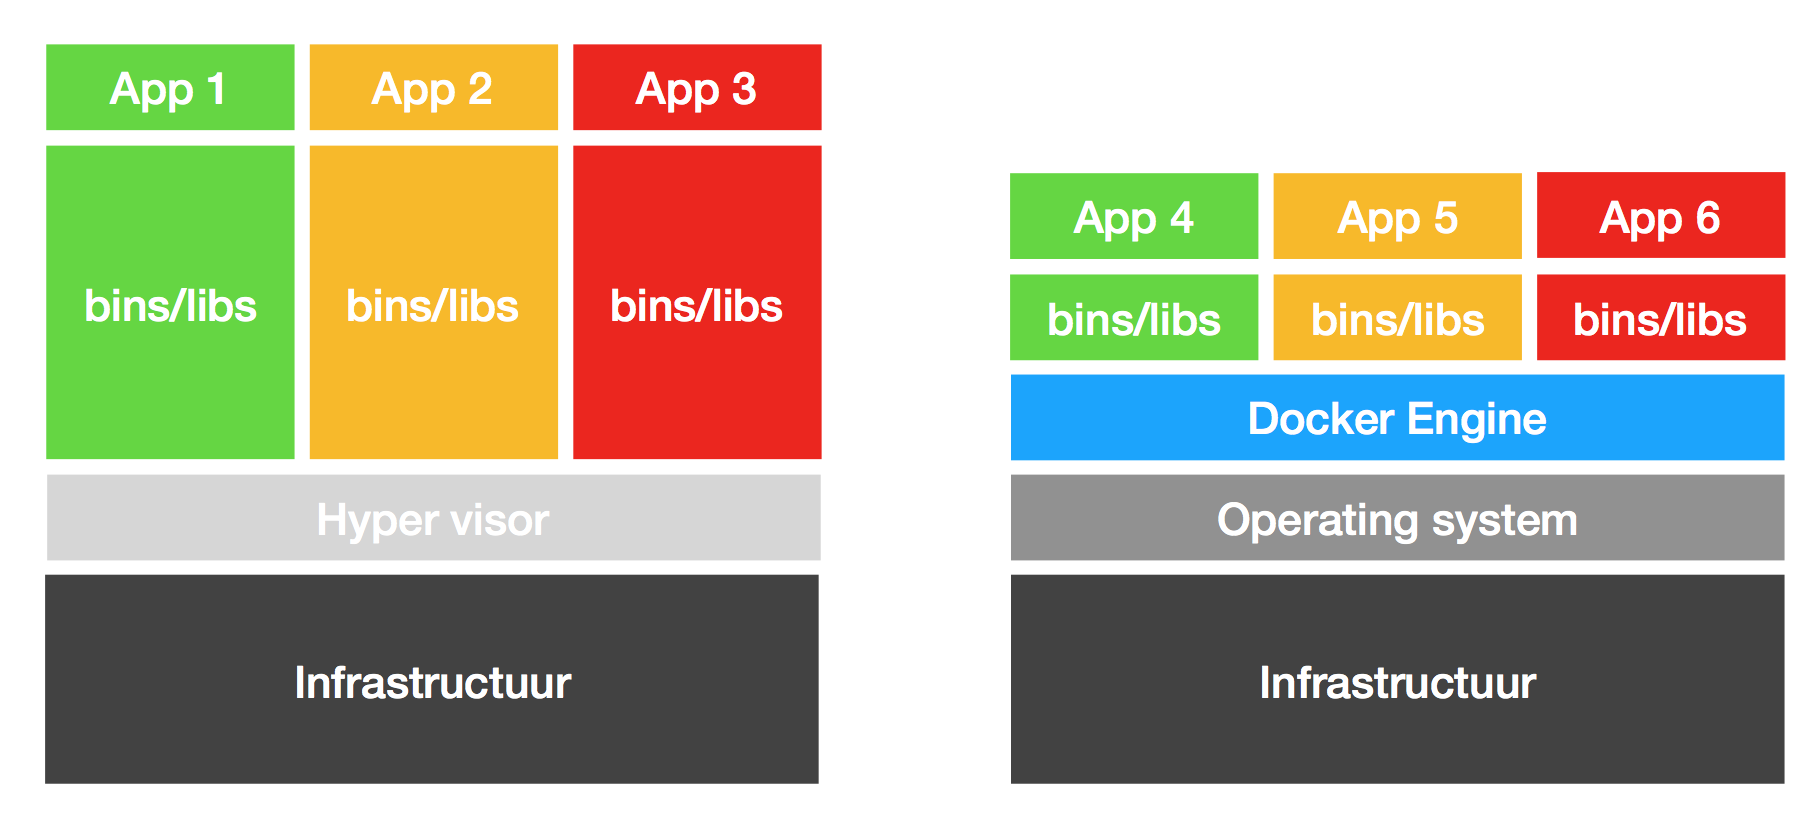
\includegraphics[height=5cm]{img/docker1.png}

Toch moeten we dit beeld met een korrel zout nemen, als we elke server gaan bekijken in termen van grootte dan zouden we het volgende beeld moeten krijgen. Aangezien we op een server met virtuele machines geen host operating system nodig hebben en we hier enkel gebruik maken van een hypervisor, is het beeld dat de hypervisor en het host operating system even groot zijn niet correct. Ook het beeld dat de docker engine even groot zou zijn als het host operating system is ook niet correct.

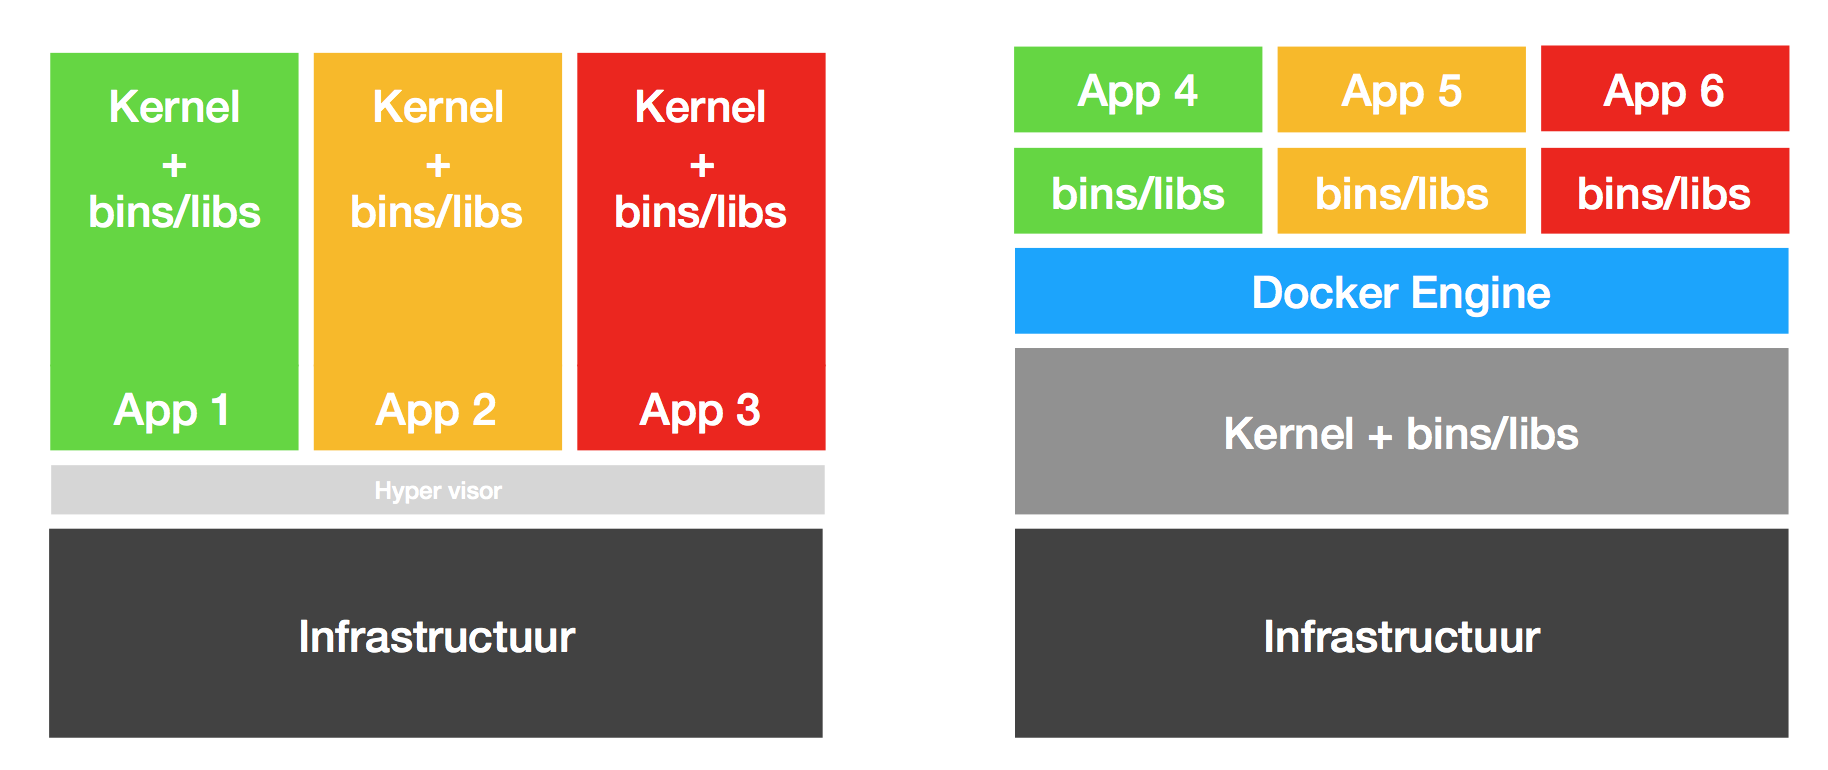
\includegraphics[height=5cm]{img/docker2.png}

Indien we alles correct zouden teken dan zien onze modellen er als volgt uit. Dit is al een representatiever beeld van een infrastructuur met virtuele machines en een infrastructuur met containers.

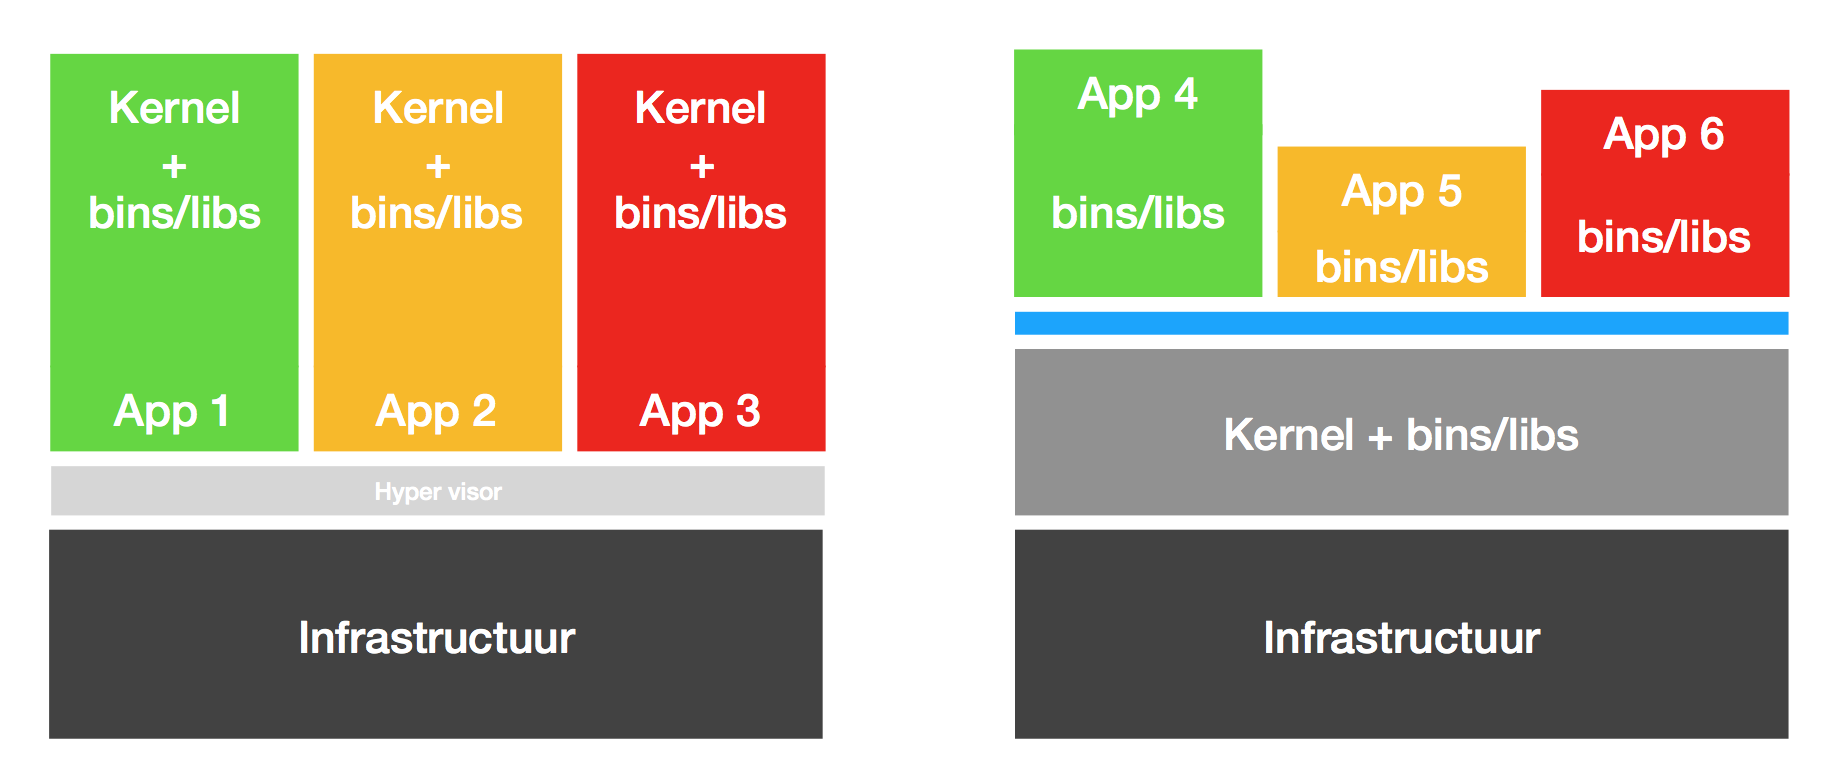
\includegraphics[height=5cm]{img/docker3.png}

Nu we het concept container wat beter begrijpen kunnen we over gaan naar de technologie die dit allemaal mogelijk maakt, namelijk Docker.

Docker is gestart in 2012 als een open source project met de originele naam dotcloud. Het doel van het project was en is om het bouwen en gebruiken van single-applications in linux containers simpeler te maken. Sindsdien is het alleen maar gegroeid in populariteit. Bovenop de abstractie die het biedt om containers aan te maken heeft docker ook een platform ontworpen dat het makkelijk maakt voor devellopers en systeembeheerders om containers te delen en te hergebruiken. Dit gedistribueerd systeem, samen met de ondersteuning op allerhande platformen heeft er voor gezorgd dat docker zo populair geworden is.

Hoe docker containers juist opgebouwd zijn alsook hoe de docker engine werkt is een bachelorproef op zich. Wel zal ik even de belangrijkste elementen aanreiken die we nodig hebben in de verdere proef.

Een Docker image is een statische specificatie van wat de container moet zijn in runtime, dit wil zeggen dat je hierin specifieert in welke folder de app moet staan, welke packages je nodig hebt, welke base image je gebruikt enz.

Van deze Docker images kan je instanties aanmaken, welke docker containers worden genoemd. Het zijn deze containers waarin onze applicatie leeft.

Er zijn er natuurlijk nog een hele hoop maar deze vallen buiten de scope van deze proef.

Zoals te zien is op foto XX zien we dat de docker engine, in tegenstelling tot een een VM-hypervisor, een operating system nodig heeft. 
Er zijn ondertussen een hand vol bedrijven bezig met het ontwerpen van operating systemen die geoptimaliseerd zijn voor het runnen van containers.
Zo heb je bijvoorbeeld VMWare die VMware Photon aan het ontwerpen zijn, of Rancher  die RancherOS Ontwerpt. Aangezien we onze virtuele machines op openstack gaan lanceren zijn we gebonden aan de VM types die zij ondersteunen. Het openstack heeft tot op de moment van het schrijven van deze proef enkel ondersteuning voor CoreOS. 

Tot op heden is CoreOS Container Linux de leider op het gebied van container operating system. Het is gebaseerd op een versie van ChromeOS en dit om het host os zo klein en simpel mogelijk het houden. 
Alle versies van CoreOs komen standaard met hun eigen container engine rtk maar ook met de Docker Engine waar wij gebruik van gaan maken.

Nu we een kleine inleiding gehad hebben over wat containers zijn en welke technologieën we ervoor gaan gebruiken, is het tijd dat we eens naar de onderliggende infrastructuur gaan kijken.

\subsection{OpenStack infrastructuur}

Zoals we in puntje 1.2 hebben kunnen vaststellen, weten we dat Combell tot op heden 2 grote platformen aanbied. Aan de ene zijde heb je de managed hosting die puur draait op VM’s en aan de aneke kant heb je hun OpenStack platform. 

Aangezien ze al een OpenStack platform hebben leek het voor hun dus ook interessanter om container clusters te gaan uitrollen op het OpenStack platform. Maar om dit tot een goed einde te brengen moeten we eerst een antwoord vinden op de vraag wat is OpenStack en hoe kunnen we het gebruiken in deze proef.

Net zoals we bij containers en VM’s gedaan hebben in puntje 1.3.1 is het niet slecht nieuwe om technologieën vanop een afstand te bekijken om te begrijpen wat ze doen en hoe ze werken.
Dit is ook wat we bij het OpenStack platform gaan doen. 

OpenStack Is een product dat ontstaan is door de samenwerking van Rackspace en het ruimtevaart agentschap NASA. Hun gezamenlijke missie was om een systeem te creeren dat het makkelijk maakte voor bedrijven om hun cloud infrastructuur (op basis van VM’s) op te zetten, maar ook om in de toekomst zonder veel moeite deze infrastructuur uit te breiden. 

Uit deze ideologie bouwde ze OpenStack. OpenStack maakt dit mogelijk omdat het ten eerste open source is en ten 2de werkt het naar analogie zoals een Linux systeem. 
Openstack is opgemaakt uit verschillende componenten. En omdat het 100% open source is is het dus ook mogelijk om bestaande componenten te wijzigen of om volledig nieuwe componenten te ontwerpen. 
Laten we even al deze mogelijkheden achterwege dan zien we dat de core van OpenStack bestaat uit 9 componenten. Elke component is verantwoordelijk voor zijn deel van de infrastructuur. Deze worden standaard geïnstalleerd bij elke installatie van OpenStack en worden onderhouden door de OpenStack Community.
Als eerste hebben we Nova, Nova is de hoofd computing engine van het Openstack Platform. Nova is verantwoordelijk voor het voor het aanmaken en managen van de VM’s.

De 2de grote component is Swift en deze is verantwoordelijk voor het opslag systeem. Om er voor te zorgen dat OpenStack de ideologie van gemakkelijk schalen kan blijven garanderen is het verwijzen naar een bestand op een bepaalde disk niet de juiste manier. Daarom zorgt Swift er voor dat programmeurs in hun code kunnen refereren naar een unieke sleutel zodat OpenStack de plaats van de file kan beslissen. Swift zorgt er op deze manier ook voor dat OpenStack de taak van het back-uppen op zich neemt. Dit is weer een zorg minder voor de ontwerpers.

Omdat in bepaalde gevallen de snelheid van gegevens belangrijker is dan de backup ervan heeft OpenStack hier ook een oplossing voor. Deze noemt Cinder, Cinder is de block storage component die programmeurs toelaat om bestanden op een bepaalde disk te raadplegen.

Een grote kracht van OpenStack is dat het ook de netwerking tussen VM’s volledig voor zijn rekening neemt. Neutron zorgt er voor dat de VM’s tegen elkaar kunnen babbeken op een gemakkelijke en efficiënte manier.

Horizon is de grafische weergave van de OpenStack cloud infrastructuur. Ook al bied OpenStack een API om de infrastructuur op te zetten (Zie later). Soms is het handig om grafisch na te gaan of alles draait naar behoren. Voor veel mensen die beginnen met OpenStack is dit het eerste aanspreekpunt.

Een volgend belangrijk aspect in een cloud infrastructuur is authenticatie en authorisatie. In OpenStack word dit behandeld door Keystone. Keystone houd een centrale lijst bij met de gebruikers die toegang hebben tot OpenStack en daarbij de rechten zie ze hebben op bepaalde services. Het is zelf zo uitgebreid dat applicatie ontwikkelaars de rechten in hun eigen applicatie kunnen weerspeigelen met de gebruikers en services van Keystone.

In OpenStack verstaan we onder “Computing engines” Virtuele machines. Zoals aangegeven in puntje 1.3.1 weten we dat OpenStack standaard een tiental VM Operating systems images bevat. Glance, de Component verantwoordelijk voor de OS Images, laat ons toe om deze images te gebruiken als templates voor het opzetten van een nieuwe virtuele machine. Deze images specifiëren onder andere welke “flavor” van Linux we wensen, welke versie, enz. Let op, in een image specifieren we niet welke recources we nodig hebben. Dit is de taak van de Heat component. 
We kunnen ons al voorstellen dat bepaalde bedrijven een eigen operating system wensen te gebruiken dat niet standaard in OpenStack aanwezig is. Daarom is er ook de optie om zelf images te schrijven. Hier gaan we niet verder op in aangezien dit buiten de scope van de proef valt.

Een OpenStack Omgeving wordt, zoals bijvoorbeeld bij Combell, opgezet om dan over te dragen aan de klant. Deze kan hier dan verder mee doen wat hij wenst. Het is dus duidelijk dat elke openstack omgeving er anders uit zal zien. Daarom hebben we Ceilometer, deze component laat ons toe om aan “Flavors” van VM’s prijzen te hangen. Zo heb je bijvoorbeeld de m1.tiny, hier krijg je 1 VCPU, 512MB RAM en een 20GB root disk. Deze kust 0.007 Euro per uur of 5 euro per maand. De beschikbare “Flavors” en hun kost, worden bepaald door de hosting provider van het OpenStack platform.

We hebben nu al een aantal keer gesproken over concept “Flavors”, en dit wordt in OpenStack mogelijk gemaakt door de Heat component. Hier kunnen we bepalen welke “Flavor” welke resources ter beschikking heeft. Welke “Flavor” de applicatieontwikkelaar kiest hangt volledig af van zijn budget en van de resources die de applicatie nodig heeft.

Wat we moeten onthouden van het OpenStack platform is dat het ons toelaat om zeer gemakkelijk, via de API of de web interface, virtuele machines te configureren en op te starten. We hoeven ons op deze manier geen zorgen te maken over de netwerk structuur als ook de beveiligde toegang tot de servers. Het laat ons ook toe om in de toekomst eenvoudig uit te breiden naar mate het verkeer naar onze servers stijgt.


\subsection{Kubernetes}

\subsection{Automatisatie}

\subsubsection{TerraForm}





\subsubsection{Ansible}

\section{Probleemstelling}

\section{Onderzoeksvragen}
\label{sec:onderzoeksvragen}

%% TODO:
%% Uit je probleemstelling moet duidelijk zijn dat je onderzoek een meerwaarde
%% heeft voor een concrete doelgroep (bv. een bedrijf).
%%
%% Wees zo concreet mogelijk bij het formuleren van je
%% onderzoeksvra(a)g(en). Een onderzoeksvraag is trouwens iets waar nog
%% niemand op dit moment een antwoord heeft (voor zover je kan nagaan).

\section{Opzet van deze bachelorproef}
\label{sec:opzet-bachelorproef}

%% TODO: Het is gebruikelijk aan het einde van de inleiding een overzicht te
%% geven van de opbouw van de rest van de tekst. Deze sectie bevat al een aanzet
%% die je kan aanvullen/aanpassen in functie van je eigen tekst.

De rest van deze bachelorproef is als volgt opgebouwd:

In Hoofdstuk~\ref{ch:methodologie} wordt de methodologie toegelicht en worden de gebruikte onderzoekstechnieken besproken om een antwoord te kunnen formuleren op de onderzoeksvragen.

%% TODO: Vul hier aan voor je eigen hoofstukken, één of twee zinnen per hoofdstuk

In Hoofdstuk~\ref{ch:conclusie}, tenslotte, wordt de conclusie gegeven en een antwoord geformuleerd op de onderzoeksvragen. Daarbij wordt ook een aanzet gegeven voor toekomstig onderzoek binnen dit domein.


%%=============================================================================
%% Methodologie
%%=============================================================================

\chapter{Methodologie}
\label{ch:methodologie}

Tijdens de bachelorproef heb ik volgende stappen ondernomen om de informatie te verzamelen, ik ben begonnen met het bepalen van de onderzoeksvraag. Nadat deze geformuleerd was ben ik begonnen met het verzamelen van de nodige informatie. De vragen die hier naar boven zijn gekomen heb ik aan de hand van een kleine interviews kunnen beantwoorden.

\section{Bepalen van de onderzoeksvraag}

Aangezien ik mijn stage doe bij Combell heb ik aan hun eerst gevraagd of zij een interessant onderwerp hadden in de wereld van de systeembeheerders. Wetende dat ze een van de grootste spelers zijn hier in België op vlak van hosting en 24/7 service moeten ze ook meegroeien met de laatste nieuwe trends. Hun infrastructuur en oplossingen voor de klant is vrij uitgebreid, daarom stelde ze me ook de vraag of ik graag iets wou doen in de systeembeheerwereld of liever iets meer hands on en dan meer gericht op de devops wereld. Ook al studeer ik af in als als systeembeheerder, toch blijf ik programmeren wel nog steeds leuk vinden. Daarom heb ik ook de optie van een opdracht in het thema devops verkozen. Na wat over en weer gemail met de mensen van het operationsteam en van het platformsteam hebben we besloten dat Combell graag een onderzoek had gevoerd naar hoe we containers kunnen integreren in het huidige aanbod. Dit met de extra moeilijkheid dat we niet alleen een simpele virtuele machine opstarten en daar Docker containers opzetten, maar dat daze ook schaalbaar moest zijn en met een zekere vorm van automatisatie. Dit was de aanzet tot de onderzoeksvraag.

\section{Literatuurstudie}

Na het bepalen van de onderzoeksvraag was het tijd om de bestaande infrastructuur in kaart te brengen en om de toekomstige technologieën te gaan onderzoeken. Aangezien ik stage deed als systeembeheerder was mijn eerste stageopdracht een algemeen beeld te vormen van wat Combell aan te bieden heeft en hoe de verschillende technologieën samen werkte. Dit was in het begin zeker geen eenvoudige opdracht aangezien alles zo uitgebreid was. Ik had dus ook een 4 tal weken nodig om me te kunnen inwerken in het hele systeem. Eenmaal ik de gebruikte technologieën verstond en mijn weg wat vond in het hele systeem kon ik beginnen aan het onderzoek. Aangezien de technologieën die ik moest gaan gebruiken vrij nieuw waren, waren er dus ook een aantal bijeenkomsten waar er uitvoerig over gesproken zou worden. Daarom leek het mij geen slecht idee om ook een te gaan luisteren op het Config Management Camp dat elk jaar doorgaat op campus Schoonmeersen van de HoGent. Hier heb ik 2 dagen een aantal talks me gevolgd die de onderwerpen Kubernetes en OpenStack aansneden. Deze gaven mij al het eerste inzicht aan wat ik me kon verwachten tijdens mijn onderzoek.

\section{Interviews}

Na het eerste onderwerp in mijn literatuurstudie namelijk de huidige infrastructuur onderzoeken, kwamen er toch een aantal vragen naar boven. Aangezien ik nog niet vertrouwd was met de technologieën die ze bij Combell hanteren, meerbepaald het OpenStack platform en VMware producten ben ik met mijn vragen bij Maarten Steenhuyse, Expert Devops Engineer, Melissa De Witte, Teamlead Systeembeheer en Wesley Hof, Team Lead Platforms gaan praten. Zij, samen met Tom Temmerman, Operations Engineer Hebben mij een zeer duidelijk antwoord kunnen bieden op de vragen betreffende de gebruikte technologieën. Deze vragen kan u vinden in Bijlage XX. Ook is het netwerk, dat deze infrastructuur nodig heeft een enorme uitdaging. Daarom ben ik ook een aantal dagen op stap geweest met Jonathan Lataire, Data Center Engineer om infrastructuur en de datacenters van dichtbij te bekijken en om een beter beeld te krijgen van hoe alles nu samen werkt. Door de ervaring en kennis van zowel het platforms team als het operations team en onze Data Center Engineer Jonathan  heb ik veel interessante en bruikbare informatie kunnen verzamelen die van groot belang waren voor het verloop van de bachelorproef.




%% Voeg hier je eigen hoofdstukken toe die de ``corpus'' van je bachelorproef
%% vormen. De structuur en titels hangen af van je eigen onderzoek. Je kan bv.
%% elke fase in je onderzoek in een apart hoofdstuk bespreken.

%\input{}
%\input{}
%...

%%=============================================================================
%% Conclusie
%%=============================================================================

\chapter{Conclusie}
\label{ch:conclusie}

%% TODO: Trek een duidelijke conclusie, in de vorm van een antwoord op de
%% onderzoeksvra(a)g(en). Wat was jouw bijdrage aan het onderzoeksdomein en
%% hoe biedt dit meerwaarde aan het vakgebied/doelgroep? Reflecteer kritisch
%% over het resultaat. Had je deze uitkomst verwacht? Zijn er zaken die nog
%% niet duidelijk zijn? Heeft het onderzoek geleid tot nieuwe vragen die
%% uitnodigen tot verder onderzoek?



\appendix

%%---------- Back matter ------------------------------------------------------

\printbibliography
\addcontentsline{toc}{chapter}{\textcolor{maincolor}{\IfLanguageName{dutch}{Bibliografie}{Bibliography}}}


\listoffigures
\listoftables

\end{document}
